\section{Wiremap}
The Wiremap is an innovative projection technique that displays a 3D image in space using a standard computer projector. The projector throws a beam of light on an array of vertical wires. From the focal point of the projector’s lens, all the wires are evenly spaced from one another and have a corresponding distance from the projector. With that information (both a horizontal and depth coordinate), and using some careful calculations on the computer, we can project simple images at various depths in the field. From any perspective besides the projector position, the wires appear randomly placed and the image becomes visible.

Our implementation uses mason's string for the field, 3/4" plywood for the top and bottom alignment/hanging boards, and standard nuts and washers as anchors for each string. Our map has 256 strings, placed in a randomized dimension of depth through an equal number of holes in both the top and bottom alignment boards. The strings are secured with bolts on the top board and weighted down with a washer below the bottom board. When the top board is raised to 8ft, the wires become taught and can be aligned to a 90 degree angle with the floor. The Wiremap must be calibrated each time the projector is positioned - this includes making sure the wires are parallel, the projector sees the wires evenly spaced, and there is no unnecessary tilt or keystone in the projector's image.

\begin{figure}[htp]\centering
  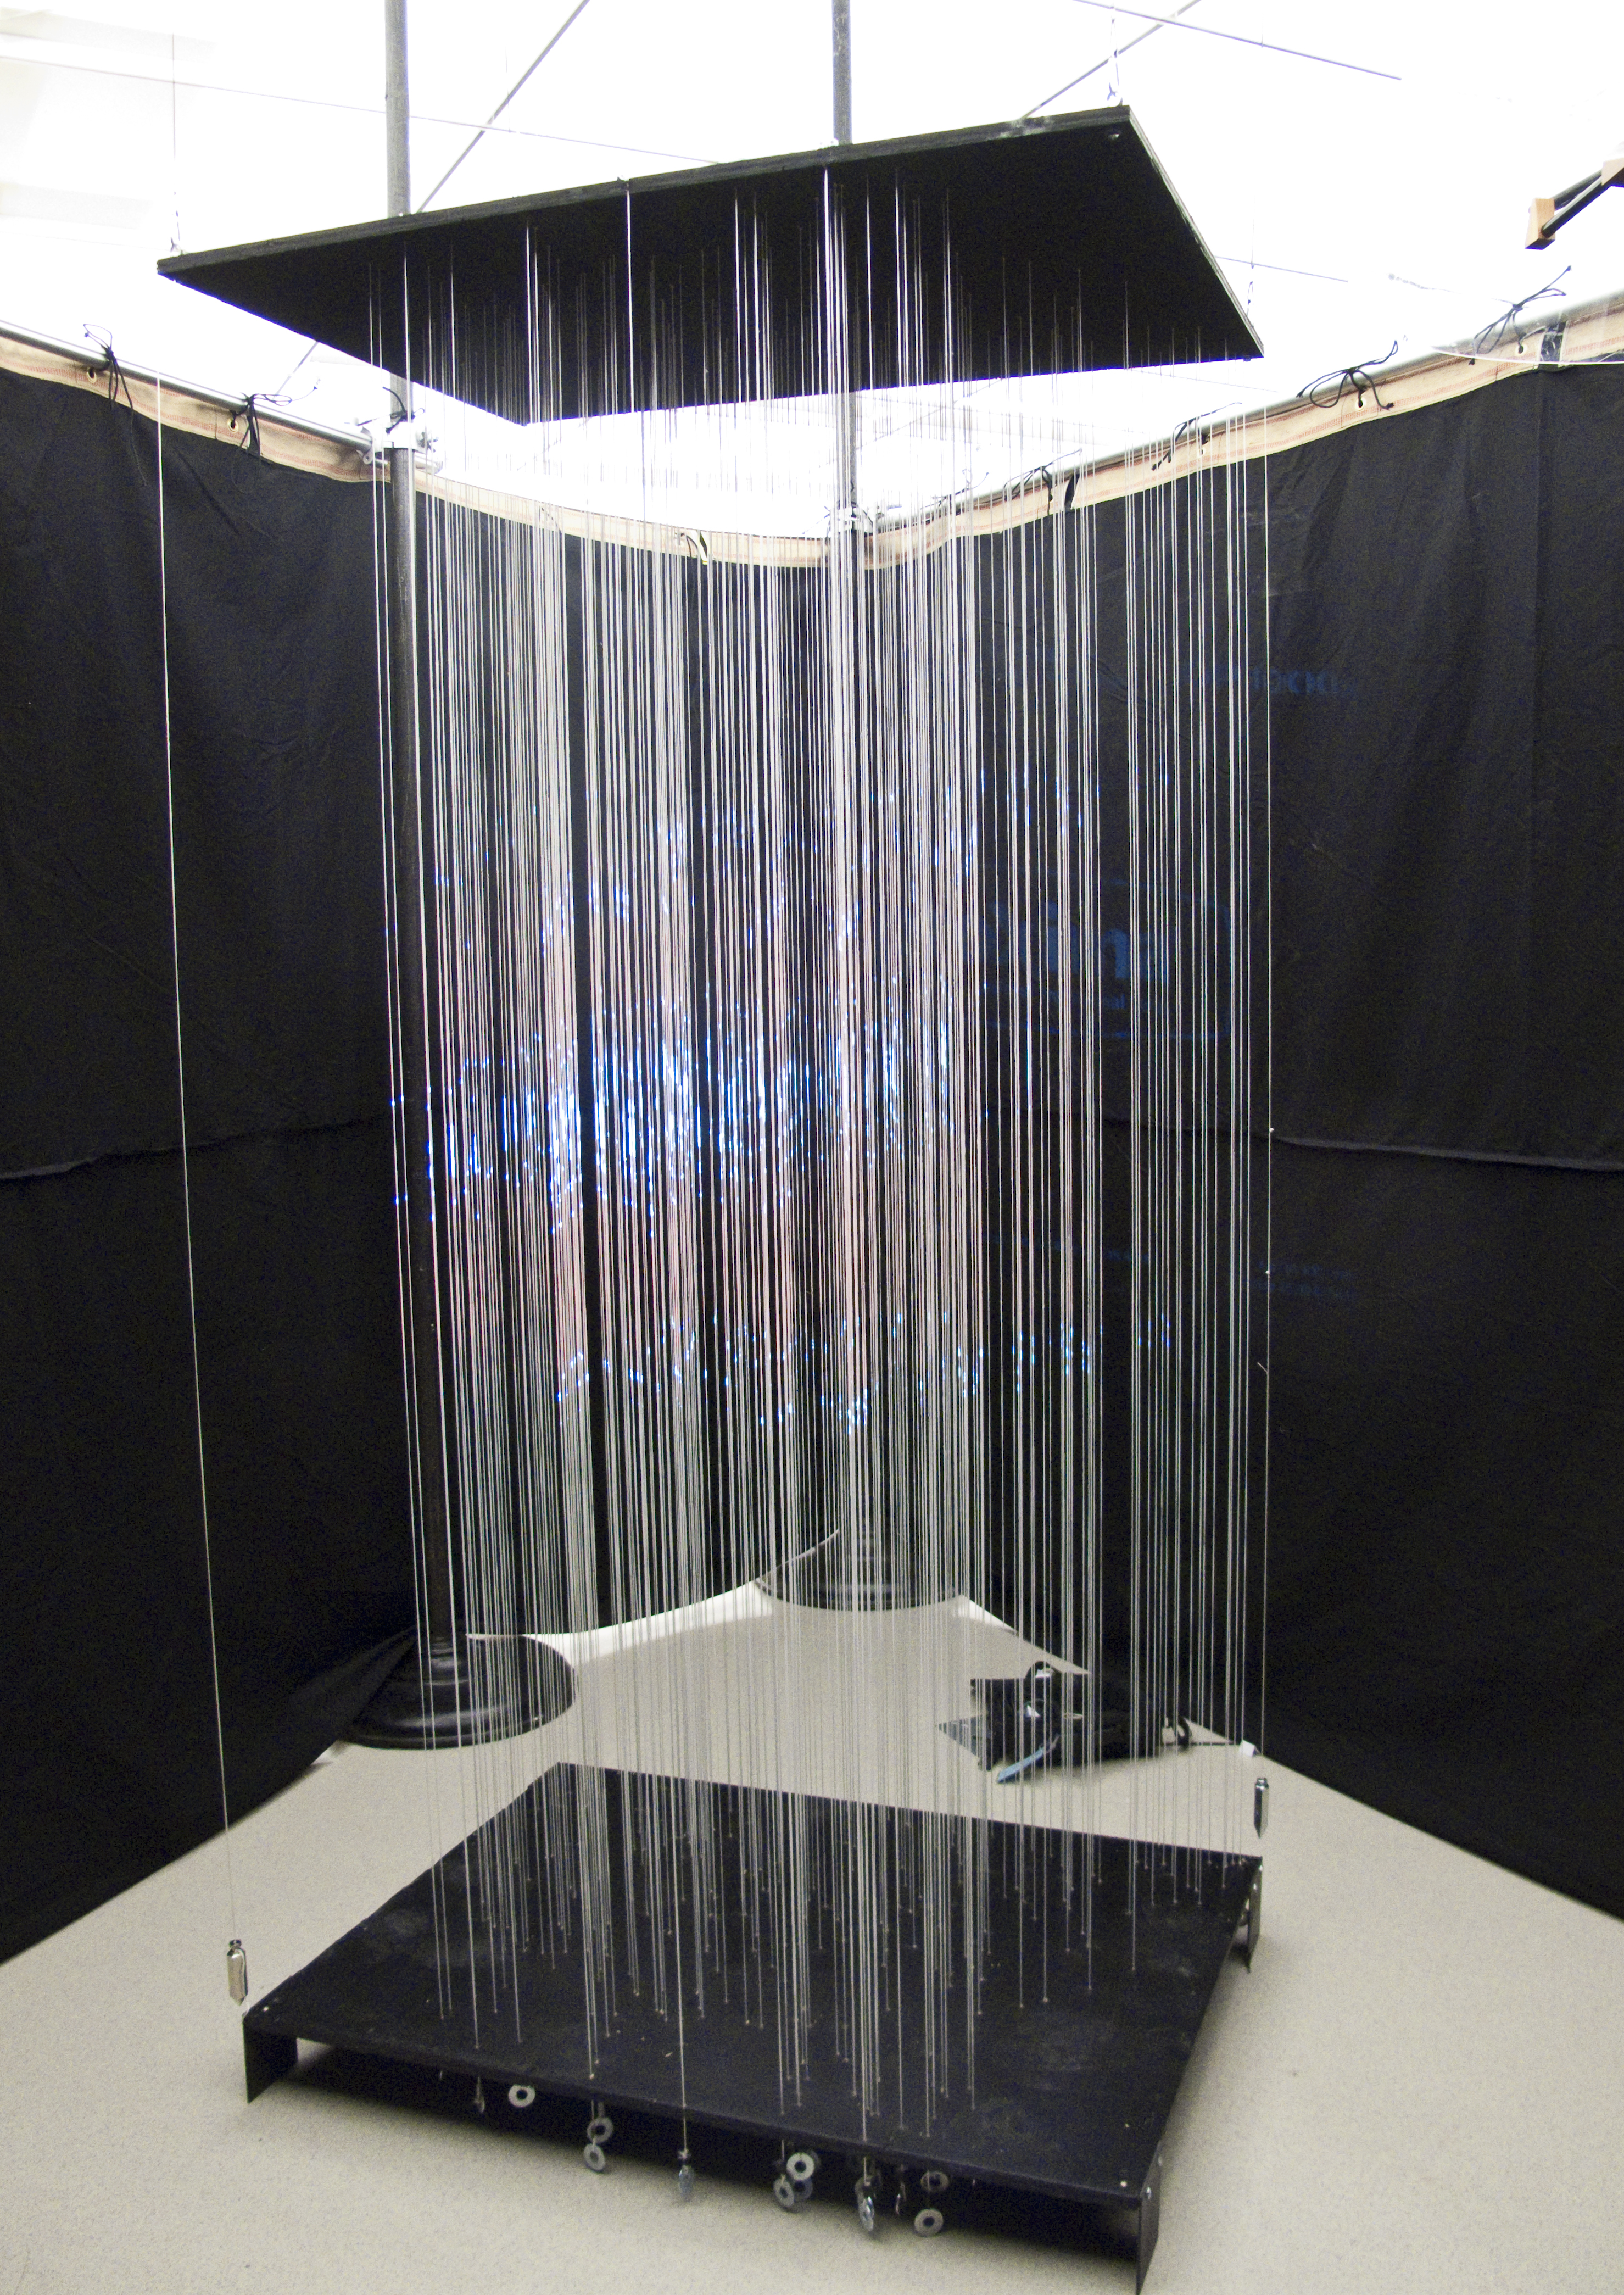
\includegraphics[width=.4\textwidth]{images/wiremapconst6.jpg}
  \caption{The 256-string Wiremap installed in the gallery.}\label{fig:wmdiagram}
\end{figure}
\subsection{Wiremap Software Library}
In order to facilitate quicker prototyping and make the Wiremap software more accessible to the team, we wrote a simple Processing library for rendering certain shapes in the Wiremap field. The library replaces the source code provided by the creator of the Wiremap \cite{AH} by reducing code duplication and abstracting most of the implementation details away from a user who wishes to simply draw a sphere, rectangle or sliver in the field. The library also includes a novel calibration method developed in response to inaccuracies in our Wiremap.

\paragraph{Abstraction}
The Wiremap library gathers the coordinate conversion and wire selection math into a single class. The previous method required duplicating a set of functions in every Processing sketch that output to the Wiremap. Now, the user creates an instance of the Wiremap class and provides a few key measurements of the physical interface as well as a text file listing the wire depths. The calculation is done as necessary, and not exposed to the user.

\paragraph{Coordinate Systems}
One key difference between the original source and the Wiremap library is the coordinate system used for each plane. Previously, the coordinates of X, Y and Z were all physical inches and matched the actual dimensions of the Wiremap. To facilitate quicker transitioning from a regular Processing sketch (using the standard 2D renderer) to one for the Wiremap, the X and Y were changed to be in the standard, Processing-style pixel coordinate system.

The Z plane remains in inches, as there is no obvious relationship between Z space on the screen (which is infinite in both directions) and Z space in the Wiremap field (limited by the physical dimensions). Thus, Z coordinates in the field range from 0 to the field depth.

\paragraph{}The library has been released under the Apache open source license, and will continue to evolve after this project's completion. See the library's documentation for details on installation and usage \cite{CP}.
